% kuleuventheme2 by Janez Kren, September 2017, janez.kren@kuleuven.be, based on:
% kuleuventheme 1.3 by Roland Pastorino, 2013 roland.pastorino@kuleuven.be / www.rolandpastorino.com

%\documentclass[11pt,t,notes=only]{beamer}
\documentclass[11pt,t]{beamer}
\usetheme[normal]{kuleuven2}	%THEME OPTIONS for LOGO: kul (default), kulak, lrd,    ; OPTIONS for TITLE PAGE: normal (default), sedes
\usepackage{multirow}

\newcommand\symO{\mathcal{O}}
\newcommand\symSA{\mathcal{SA}}
\newcommand\symSAH{SAH}
\newcommand\symCost{\mathcal{K}}
\newcommand\symLeft{l}
\newcommand\symRight{r}
\newcommand\symNbPrimitives{n}
\newcommand\symIntersection{i}
\newcommand\symTraversal{d}
\newcommand\symTraversalL{\expandafter\MakeUppercase\expandafter{\symTraversal}}
\newcommand\symNodeExample{p}
\newcommand\symLeaf{b}
\newcommand\symLeafL{\expandafter\MakeUppercase\expandafter{\symLeaf}}
\newcommand\symTime{T}
\newcommand\symRender{render}
\newcommand\symTotal{totaal}
\newcommand\symInternal{inwendig}
\newcommand\symBSP{BSP}
\newcommand\symKd{Kd}
\newcommand\symCostTraversalBSP{\symCost_{\symTraversal,\symBSP}}
\newcommand\symCostTraversalKd{\symCost_{\symTraversal,\symKd}}
\newcommand\symCostTraversal{\symCost_{\symTraversal}}
\newcommand\symRandom{random}
\newcommand\symBSPrandom{\symBSP_{\symRandom}}
\newcommand\symBSPrandomkd{\symBSP_{\symRandom+}}
\newcommand\symBSPrandomfastkd{\symBSP^{\symKd}_{\symRandom+}}
\newcommand\symBSPrandomsomekd{\symBSP^{(\symKd)}_{\symRandom+}}
\newcommand\symBSPrandomany{\symBSP^{(\symKd)}_{\symRandom(+)}}
\newcommand\symArbitrary{wn}
\newcommand\symBSParbitrary{\symBSP_{\symArbitrary}}
\newcommand\symBSParbitrarykd{\symBSP_{\symArbitrary+}}
\newcommand\symBSParbitraryfastkd{\symBSP^{\symKd}_{\symArbitrary+}}
\newcommand\symBSParbitrarysomekd{\symBSP^{(\symKd)}_{\symArbitrary+}}
\newcommand\symBSParbitraryany{\symBSP^{(\symKd)}_{\symArbitrary(+)}}
\newcommand\symCluster{cn}
\newcommand\symBSPcluster{\symBSP_{\symCluster}}
\newcommand\symBSPclusterkd{\symBSP_{\symCluster+}}
\newcommand\symBSPclusterfastkd{\symBSP^{\symKd}_{\symCluster+}}
\newcommand\symBSPclustersomekd{\symBSP^{(\symKd)}_{\symCluster+}}
\newcommand\symBSPclusterany{\symBSP^{(\symKd)}_{\symCluster(+)}}
\newcommand\symBSPize{\symBSP_{IZE}}
\newcommand\symBSPizefastkd{\symBSP^{\symKd}_{IZE}}
\newcommand\symBSPKd{\symBSP^{\symKd}}
\newcommand\symBSPsweep{\symBSP_{SWEEP}}
\newcommand\symBSPsweepkd{\symBSP^{\symKd}_{SWEEP}}
\newcommand\symBSPsweepmaybewithkd{\symBSP_{SWEEP(+)}}
\newcommand\symMaxPrims{\symNbPrimitives_{max}}
\newcommand\symMaxDepth{d_{max}}


\newcommand\symBVH{BVH}
\newcommand\symRBSP{RBSP}
\newcommand\symRBSPKd{RBSP^{\symKd}}
\newcommand\symRBSPsomekd{RBSP^{(\symKd)}}
\newcommand\symKDOP{k-DOP}

\newcommand\authorKammaje{Kammaje en Mora}
\newcommand\authorIze{Ize et al}
\newcommand\authorGoldsmithSalmon{Goldsmith en Salmon}
\newcommand\authorMacDonaldBooth{MacDonald en Booth}
\newcommand\authorHavran{Havran}
\newcommand\authorBudge{Budge et al}
\newcommand\authorZachmann{Zachmann}
\newcommand\authorKlosowki{Klosowski et al}
\newcommand\authorHavranBittner{Havran en Bittner}
\usepackage{color}
\usepackage{tikz-qtree}
\definecolor{nodeblue1}{HTML}{44FFFF}
\definecolor{nodeblue2}{HTML}{2D00AF}
\definecolor{nodered1}{HTML}{DF2D00}
\definecolor{nodered2}{HTML}{FF4488}
\definecolor{nodered3}{HTML}{EF5D00}
\definecolor{nodered4}{HTML}{FF8888}
\definecolor{nodeyellow1}{HTML}{FFFF00}
\usepackage{subcaption}

%%% OTHER SETTINGS
\usefonttheme[onlymath]{serif}			% math font with serifs, delete to make it sans-serif
\setbeamertemplate{footline}[body] 		% delete this line to remove footline bar on all frames
%\usepackage[orientation=landscape,size=custom,width=16,height=9,scale=0.5,debug]{beamerposter} %enable for widescreen 16:9 ratio
%\titlegraphic{ \includegraphics[width=.2\paperwidth]{mytitlepagepic.png} } %optional title page image


%%% ADDED PACKAGES:
\usepackage[dutch]{babel}
\usepackage{amsfonts}
\usepackage{amssymb}


%%% TITLE PAGE INFO:
\title[Het gebruik van de normalen bij het bouwen van $\symBSP$ acceleratiestructuren]{Het gebruik van de normalen bij het bouwen van BSP acceleratiestructuren} %[]] will appear in footline
\subtitle{Thesisverdediging}

\author{Jesse Hoobergs}
\institute{KU Leuven}
\date{Juni 2019}




\begin{document}
\csname beamer@calculateheadfoot\endcsname %recalculate head and foot dimension


 %%
 %%  0. TITLE PAGE and TABLE OF CONTENT
 %%
% Title page
\begin{frame}[plain,noframenumbering]
	\titlepage
\end{frame}
	

% Table of Contents
\begin{frame}{Overzicht}
	\hfill	{\large \parbox{.961\textwidth}{\tableofcontents[hideothersubsections]}}
\end{frame}







 %%
 %%  SECTION 1 - Inleiding
 %%
\section{Inleiding}
\begin{frame}{Ray tracing}  %option fragile needed for verbatim environment
\begin{itemize}
	%\item \texttt{kul} \qquad (default, used if no option is specified) 
\includegraphics[height=.05\paperheight]{graphics/KUL.pdf}
	\item Fysisch gebaseerd renderen
	\item Stralen volgen door een scene
\end{itemize}
\pause
\vspace{5pt}
\hspace{5pt}
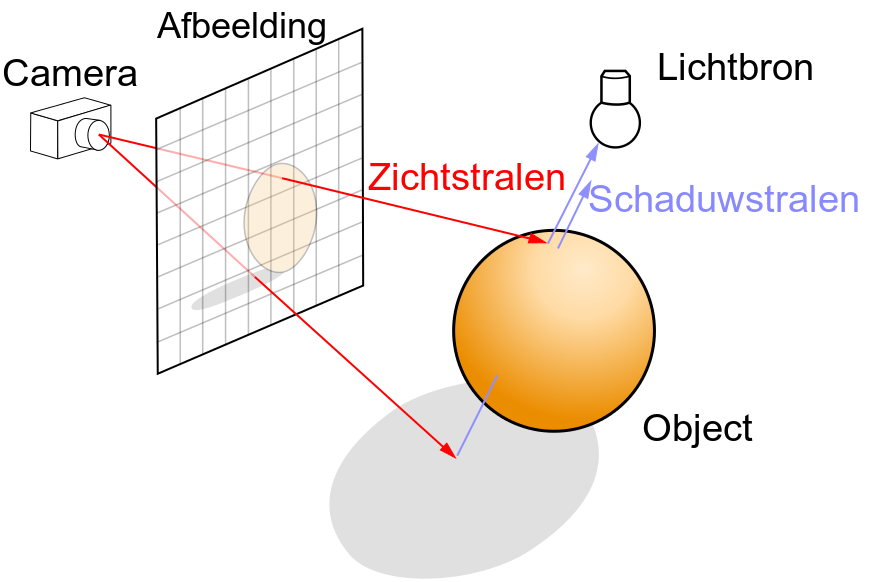
\includegraphics[height=.6\paperheight]{../img/ray-tracing}
%\vspace{24pt}

\end{frame}

\note{Ray tracing is een computergrafiek techniek voor fysisch gebaseerd renderen. 
Het doel is om realistische afbeeldingen te genereren door stralen te volgen door de scene.
\\
(click)\\
Een virtuele camera en een afbeeldingsvlak worden in de scene geplaatst.
Vanuit deze virtuele camera worden zogenaamde zichtstralen gestuurd doorheen de pixels.
Voor elke van deze stralen wordt het eerste intersectiepunt met de scene gezocht.
De kleur van de pixel komt overeen met de kleur van het intersectiepunt.\\
Om directe belichting, dit is licht dat rechtstreeks vanuit de lichtbron op het intersectiepunt valt, 
in rekening te brengen, wordt gebruikt gemaakt voor schaduwstralen.
Dit zijn stralen die vanuit het intersectiepunt naar de lichtbron gestuurd worden.
Via deze stralen kan bepaald worden of de lichtbron afgeschermd is of niet.
Een belangrijk verschil tussen zichtstralen en schaduwstralen is dat zichtstralen het eerste intersectiepunt zoeken
en schaduwstralen eender welke intersectiepunt dichter dan de lichtbron.\\
De objecten in de ruimte worden vaak voorgesteld door triangle meshes, een verzameling driehoeken.
De intersecties tussen de stralen en de scene komen dan neer op straal-driehoekintersecties.
}


\begin{frame}{Ray tracing}  %option fragile needed for verbatim environment
\begin{itemize}
	\item Praktische aantallen:
\begin{itemize}
	\item 1 miljoen pixels
	\item 1 miljoen driehoeken (mogelijks veel meer)
	\item 100 stralen per pixel
\end{itemize}
\end{itemize}
\vspace{20pt}
\pause
$\implies 10^{14}$ straal-driehoekintersecties\\
\pause
\vspace{20pt}
$\implies$ Acceleratiestructuren

\end{frame}

\note{
	In de praktijk zijn er vaak meer dan een miljoen pixels en scenes met meer dan een miljoen driehoeken zijn ook zeer normaal.
	In plaats van één zichtstraal per pixel worden honderden zichtstralen gestuurd per pixel tegen aliasing en ruis.
	\\ 
	(click) \\
	Dit komt neer op tien tot de veertiende straal-driehoekintersecties een niet haalbaar groot aantal.
	\\
	(click) \\
	Om dit probleem op te lossen, is er nood aan acceleratiestructuren
}

\begin{frame}{Acceleratiestructuren}
	\begin{itemize}
		\item Doel:
		\begin{itemize}
			\item Totale rendertijd minimaliseren
			\item Straal-driehoekintersecties te verminderen
		\end{itemize}
		\pause
		\item Simpelste versie
		\begin{itemize}
			\item Omhullende volume van scene (balk, bol, etc)
			\item Test intersectie met omhullend volume
				\begin{itemize}
					\item \texttt{Intersectie}: \qquad\qquad Test alle driehoeken
					\item \texttt{Geen intersectie}: \qquad Test nul driehoeken
				\end{itemize}
			\item Recursief opdelen tot boomstructuur
		\end{itemize}
		\pause
		\item Twee manieren van opdelen:
			\begin{itemize}
				\item Volgens objecten
				\item Volgens volume
			\end{itemize}
	\end{itemize}

\end{frame}

\begin{frame}{Opdelen volgens object}
	\begin{itemize}
		\item Driehoeken opgedeeld in disjuncte groepen
		\item Kindvolumes = omhullende volumes groepen
		\item Elke driehoek in exact één kindvolume
		\item Kindvolumes kunnen overlappen in de ruimte
	\end{itemize}
	\pause
	\vspace{5pt}
	\hspace{20pt}
	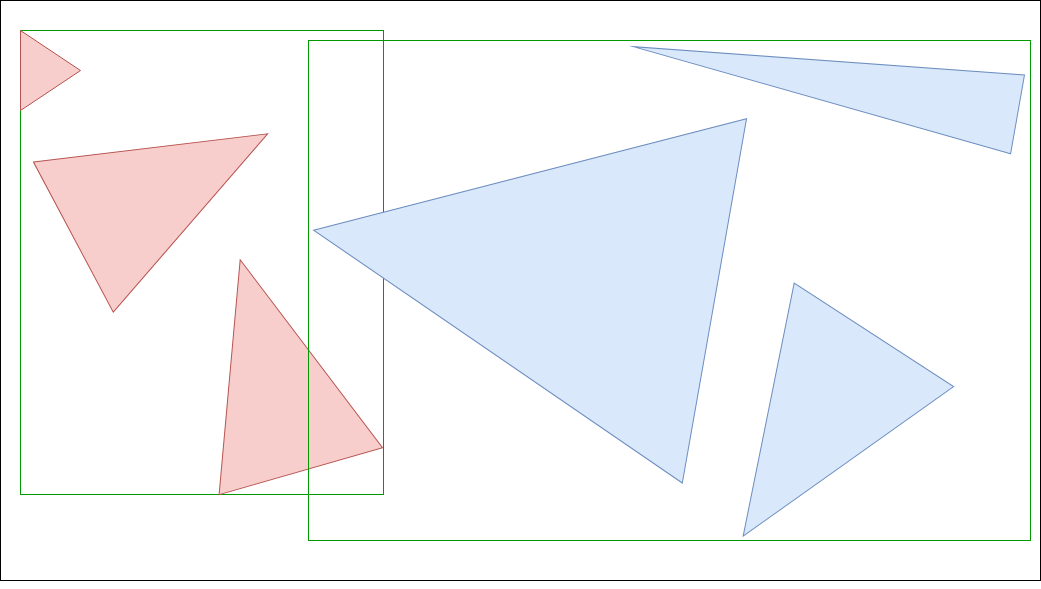
\includegraphics[height=.4\paperheight]{../img/objectSplit}
\end{frame}

\begin{frame}{Opdelen volgens ruimte}
	\begin{itemize}
		\item Volume opgedeeld in disjuncte groepen
		\item Splitsing via \textit{splitsingsvlakken}
		\item Elke driehoek in minstens één kindvolume
		\item Kindvolumes overlappen niet in de ruimte
	\end{itemize}
	\pause
	\vspace{5pt}
	\hspace{20pt}
	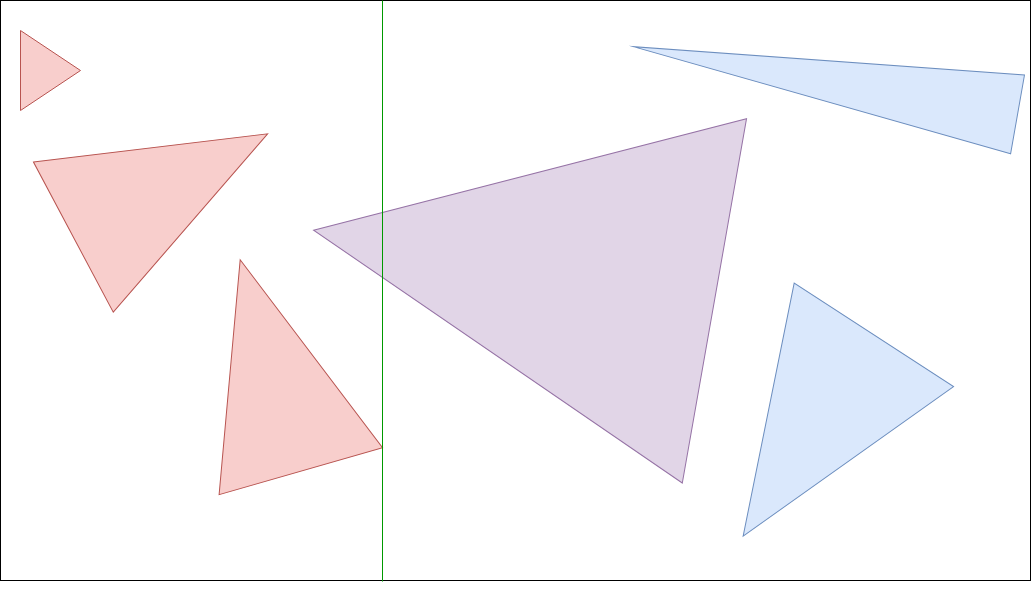
\includegraphics[height=.4\paperheight]{../img/volumeSplit}
\end{frame}

\begin{frame}{$\symBSP$ bomen}
	\begin{itemize}
		\item \textit{Binary Space Partitioning} bomen
		\item Delen volgens ruimte
		\item Delen steeds in 2 kindvolumes
		\item Splitsing via willekeurige vlakken in de ruimte
		\item $\symKd$ boom:
			\begin{itemize}
				\item Enkel asgealigneerde vlakken
				\item Computationele voordelen bij bouwen en renderen
				\item Meest gebruikte $\symBSP$ boom
			\end{itemize}
		\item Algemene $\symBSP$ boom:
			\begin{itemize}
				\item Veel meer mogelijke splitsingsvlakken
				\item Moeilijk om goede te vinden
			\end{itemize}			
	\end{itemize}
\end{frame}

\begin{frame}{Doel thesis}
	\begin{itemize}
		\item Algemene $\symBSP$ boom
		\item Normalen van driehoeken
		\item Goede splitsingsvlakken
	\end{itemize}
	\vspace{10pt}
	\begin{itemize}
		\item $\symBSPsweep$ boom
	\end{itemize} 
\end{frame}


 %%
 %%  SECTION 2 - BSP-bomen
 %%
 \section{$\symBSP$ bomen}

 \begin{frame}{$\symBSP$ bomen}
	\begin{itemize}
		\item Bouwen
		\item Intersecteren
		\item Bestaande $\symBSP$ bomen
	\end{itemize}
\end{frame}

\begin{frame}{Bouwen $\symBSP$ boom}
	\begin{itemize}
		\item Wortelknoop
		\begin{itemize}
			\item Volume = omhullende balk scene
			\item Bevat alle driehoeken
		\end{itemize}
		\item Splits in twee kindknopen
		\begin{itemize}
			\item Splits het volume volgens een splitsingsvlak
			\item Maak twee kindknopen, één voor elk volumedeel
			\item Bepaal voor elke kindknoop de driehoeken
		\end{itemize}
		\item Splits kindknopen recursief tot stopconditie
	\end{itemize}
\end{frame}

\begin{frame}[c]{Bouwen $\symBSP$ boom}
	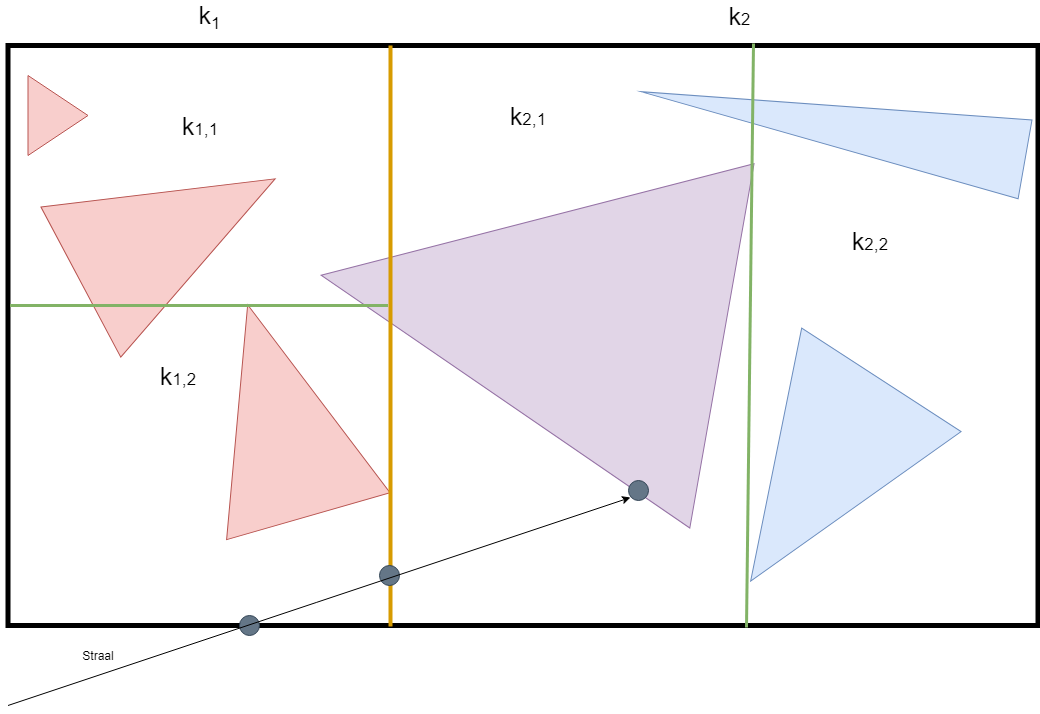
\includegraphics[width=0.8\paperwidth]{../img/volumeSplitTraversal}
\end{frame}

\begin{frame}{Intersecteren $\symBSP$ boom}
	\begin{itemize}
		\item Bepaal intersectie straal met wortelknoop:
			\begin{itemize}
				\item geen intersectie: geen intersecterende driehoek
				\item anders: doorkruis de wortelknoop
			\end{itemize}
		\item Doorkruisen knoop 
			\begin{itemize}
				\item Inwendige knoop
					\begin{itemize}
						\item Bepaal intersectie straal met splitsingsvlak
						\item Bepaal de volgorde waarin de straal door de kindknopen gaat
						\item Doorkruis de kindknopen in deze volgorde
					\end{itemize}
				\item Bladknoop
					\begin{itemize}
						\item Bepaal voor elke driehoek de straal-driehoek intersectie
					\end{itemize}
			\end{itemize}
	\end{itemize}
\end{frame}

\begin{frame}[c]{Intersecteren $\symBSP$ boom}
	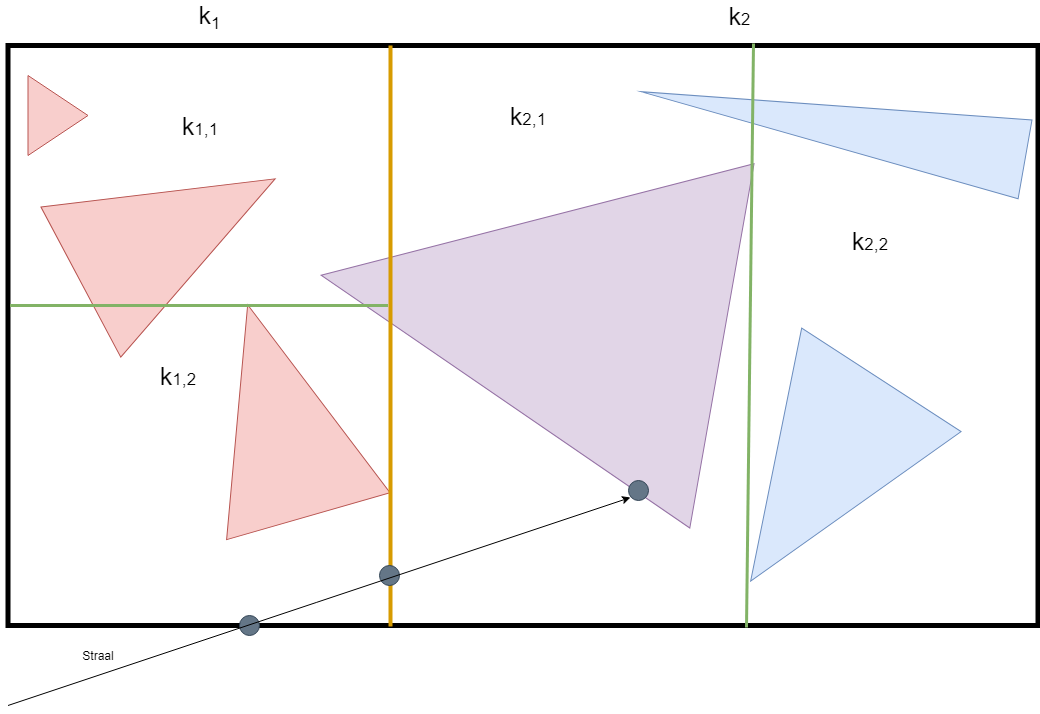
\includegraphics[width=0.8\paperwidth]{../img/volumeSplitTraversal}
\end{frame}

\begin{frame}{$\symKd$ boom}
	\begin{itemize}
	\item Enkel asgealigneerde splitsingsvlakken
		\begin{itemize}
			\item Volume elke knoop = asgealigneerde balk
			\item Goedkoper doorkruisen inwendige knoop
			\item Kunnen zich minder goed aanpassen aan scene
		\end{itemize}
	\end{itemize}
	\pause
	\vspace{5pt}
	\hspace{5pt}
	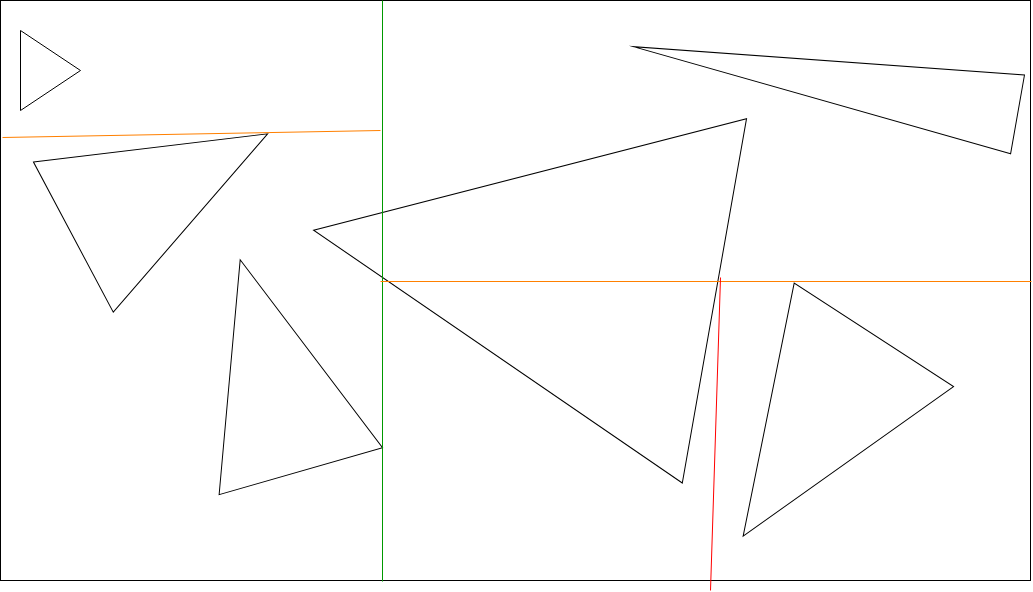
\includegraphics[height=0.5\paperheight]{../img/splitsing-Kd}

\end{frame}

\begin{frame}{Bepalen beste splitsingsvlak}
	\begin{itemize}
	\item Bepaal kost na splitsen volgens vlak
	\item Kies beste splitsingsvlak of splits niet
	\pause
	\item \textit{Surface Area} heuristiek
		\begin{itemize}
			\item Kans om kindknoop te doorkruisen is evenredig met oppervlakte
			\item Kost knoop evenredig met aantal driehoeken
			\item Na splitsing zijn beide kindknopen bladknopen
			\item $\symCost_\symNodeExample = \frac{\symSA(\symLeft)}{\symSA(\symNodeExample)}*\symNbPrimitives_\symLeft*\symCost_\symIntersection + \frac{\symSA(\symRight)}{\symSA(\symNodeExample)}*\symNbPrimitives_\symRight*\symCost_\symIntersection + \symCost_\symTraversal$
			\item Kost om niet te splitsen: $\symNbPrimitives_\symLeft*\symCost_\symIntersection$
		\end{itemize}
	\pause
	\item Alle asgealigneerde vlakken testen is onhaalbaar
		\begin{itemize}
			\item Havran: slechts $2n$ mogelijke splitsingsvlakken per richting
			\item $\symSA$ kost stijgt/daalt monotoon tussen eindpunten driehoeken langs die richting
			\item Enkel asgealigneerde vlakken door eindpunten testen
		\end{itemize}
	\end{itemize}
\end{frame}

\begin{frame}{Bepalen beste splitsingsvlak}
	\begin{itemize}
		\item $\symSA$ kost berekenen
			\begin{itemize}
				\item Aantal driehoeken in beide kindknopen nodig
				\item Oppervlaktes beide kindknopen nodig
			\end{itemize}
		\pause
		\item \textit{Sweeping}
			\begin{itemize}
				\item Sorteer driehoeken volgens eindknopen langs as
				\item 'Veeg' over de as en update $n_l$ en $n_r$
			\end{itemize}
	\end{itemize}
	\vspace{5pt}
	\hspace{10pt}
	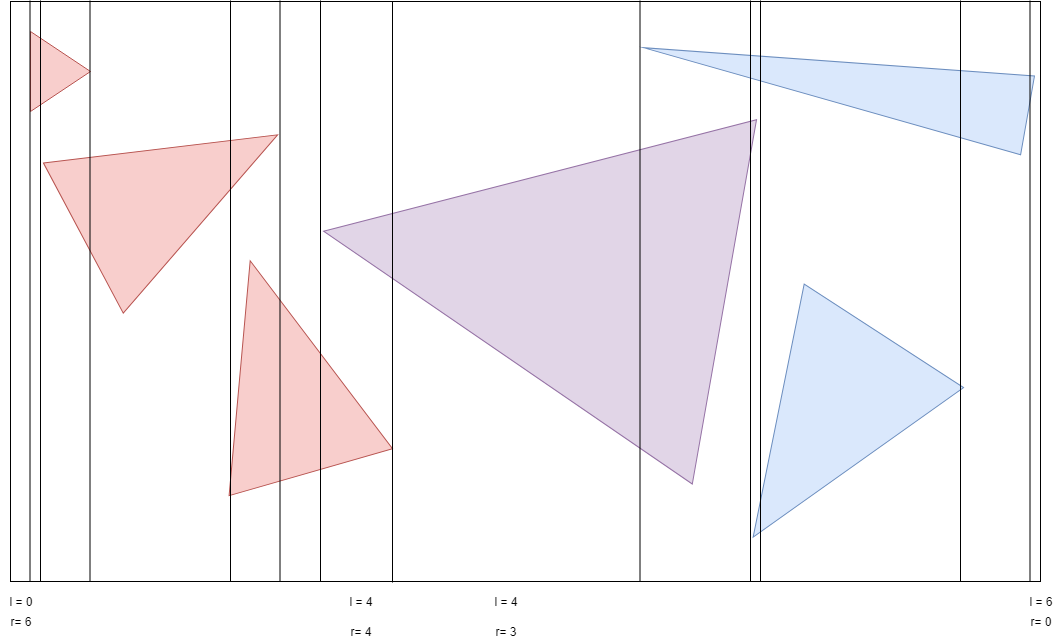
\includegraphics[height=0.45\paperheight]{../img/sweep}
\end{frame}

\begin{frame}{$\symRBSP$ boom}
	\begin{itemize}
		\item Enkel splitsingsrichtingen uit vaste verzameling van k richtingen
			\begin{itemize}
				\item Volume elke knoop = $\symKDOP$
				\item Duurder doorkruisen inwendige knoop
				\item Kunnen niet alle niet-intersecterende driehoeken scheiden
			\end{itemize}
	\end{itemize}
	\pause
	\vspace{5pt}
	\hspace{5pt}
	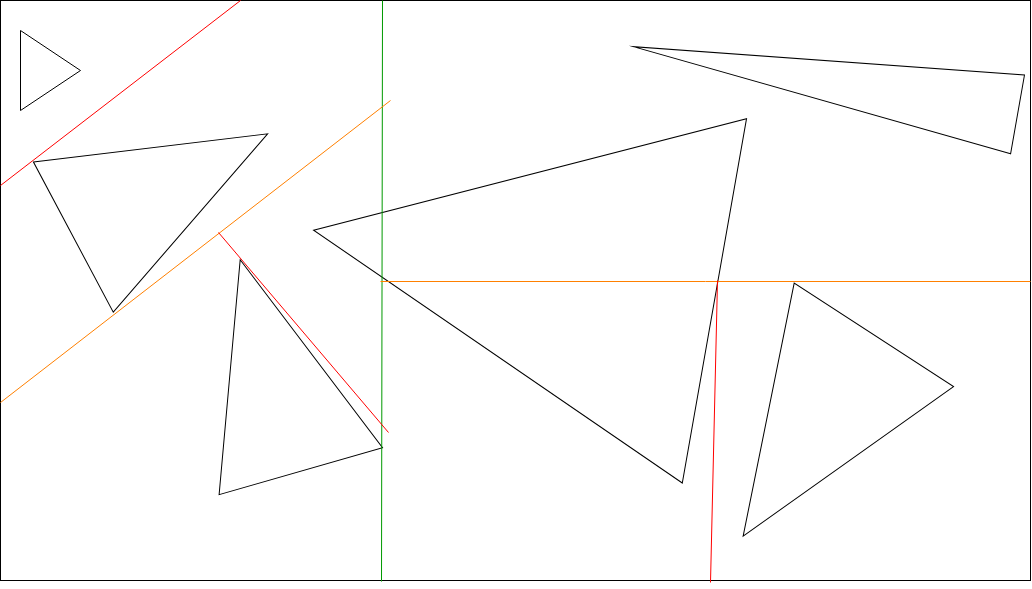
\includegraphics[height=0.5\paperheight]{../img/splitsing-RBSP}
\end{frame}

\begin{frame}{Praktisch}
	\begin{itemize}
	\item Bepalen vaste verzameling splitsingsrichtingen
	\begin{itemize}
		\item Belangrijk dat ze samen de eenheidsbol goed bedekken
	\end{itemize}
	\item $\symSA$ kost kan gebruikt worden, inclusief \textit{sweeping}
	\item Oppervlakte $\symKDOP$ berekenen is duurder
	\item Ten opzichte van $\symKd$ boom
		\begin{itemize}
			\item Minder straal-driehoekintersecties
			\item Tragere inwendige knoopdoorkruising
			\item Tragere rendertijd
		\end{itemize}
	\end{itemize}
\end{frame}

\begin{frame}{$\symBSPize$ boom}
	\begin{itemize}
	\item Enige bestaande algemene $\symBSP$ boom bij rendering
	\item Geometrie-afhankelijke splitsingsvlakken
		\begin{itemize}
			\item De asgealigneerde vlakken van $\symKd$ boom
			\item Vlak door elke driehoek
			\item Drie vlakken door zijde driehoek en loodrecht op driehoek
		\end{itemize}
	\item Volume elke knoop = convex veelvlak
	\item Sweeping
		\begin{itemize}
			\item Mogelijk voor de $\symKd$ richtingen
			\item Niet mogelijk voor de vier andere vlakken per driehoek
			\begin{itemize}
				\item $\symBVH$ hulpstructuur nodig om $n_l$ en $n_r$ efficiënt te berekenen
				\item Tragere bouwtijd
			\end{itemize}
		\end{itemize}
	\end{itemize}
\end{frame}

\begin{frame}{$\symBSPizefastkd$ boom}
	\begin{itemize}
	\item Optimalisatie
	\pause
	\item Inwendige $\symKd$ knopen bevoordelen
		\begin{itemize}
			\item Sneller te doorkruisen dan $\symBSP$ knopen
			\item Lagere doorkruiskost in $\symSA$ kost dan inwendige $\symBSP$ knopen
		\end{itemize}
	\pause
	\item Aanpassing $\symSA$ heuristiek
		\begin{itemize}
			\item Aparte $\symCostTraversalKd$ en $\symCostTraversalBSP$
			\pause
			\item Rechtstreeks gebruiken in $SA$ kost werkt niet
			\begin{itemize}
				\item $SA$ kost varieert lineair in aantal driehoeken
				\item $\symBSP$ knopen splitsen beter
				\item Bijna enkel $\symBSP$ knopen gebruikt
			\end{itemize}
			\pause
			\item $\symCostTraversalBSP$ lineair afhankelijke van aantal driehoek
			\begin{itemize}
				\item $\symCostTraversalBSP = \alpha * \symCost_\symIntersection * (\symNbPrimitives - 1) + \symCostTraversalKd$
				\item Beste splitsingsvlak zoeken
				\item Indien niet gevonden, vaste $\symCostTraversalBSP$
			\end{itemize}
		\end{itemize}
	\end{itemize}
\end{frame}

\begin{frame}{Vergelijking}
	\begin{itemize}
	\item Ten opzichte van $\symKd$ boom
		\begin{itemize}
			\item Geen volledige sweeping mogelijk
			\item Minder straal-driehoekintersecties
			\item Gemiddeld lichtjes tragere inwendige knoopdoorkruising
			\item Lichtjes snellere rendertijd
		\end{itemize}
	\pause
	\item Ten opzichte van $\symRBSP$ boom
		\begin{itemize}
			\item Duurdere bouwtijd
			\item Beide kunnen snelle $\symKd$ doorkruising gebruiken
		\end{itemize}
	\end{itemize}
\end{frame}

\begin{frame}{Vergelijking}
	\begin{itemize}
		\item Aantal splitsingsvlakken per niveau
		\begin{itemize}
			\item $\symKd$: $6n$
			\item $\symRBSP$: $2kn$
			\item $\symBSPize$: $10n$
		\end{itemize}
		\item Totaal aantal verschillende geteste splitsingsvlakken
		\begin{itemize}
			\item $\symKd$: $6n$
			\item $\symRBSP$: $2kn$
			\item $\symBSPize$: $10n$ 
		\end{itemize}
		\item Zelfs $\symBSPize$ gebruikt niet volledige vrijheid
	\end{itemize}
\end{frame}

\begin{frame}{Aantal splitsingsvlakken}
	\begin{itemize}
		\item Zelfde splitsingsvlakken op elk niveau (bv $\symBSPize$)
	\end{itemize}
	\resizebox{0.8\textwidth}{!}{%
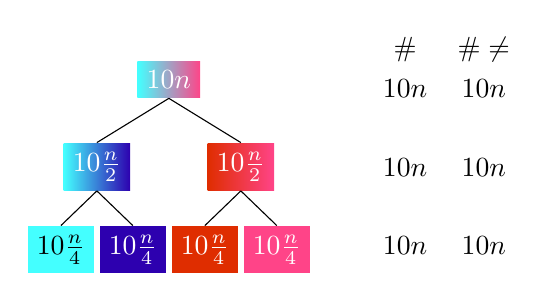
\begin{tikzpicture}
\Tree
[ .\node[shading = axis, left color=nodeblue1, right color=nodered2,shading angle=90, text=white]{$10n$};    
[.\node[shading = axis, left color=nodeblue1, right color=nodeblue2,shading angle=90, text=white]{$10\frac{n}{2}$};
 [.\node(n3l)[fill=nodeblue1]{$10\frac{n}{4}$};]
 [.\node[fill=nodeblue2, text=white]{$10\frac{n}{4}$};]
]
[.\node[shading = axis, left color=nodered1, right color=nodered2,shading angle=90, text=white]{$10\frac{n}{2}$};
 [.\node[fill=nodered1, text=white]{$10\frac{n}{4}$};]
 [.\node(n3r)[fill=nodered2, text=white]{$10\frac{n}{4}$};]
]
]
\node at (3,0.5) {$\#$};
\node at (4,0.5) {$\# \neq$};
\node at (3,0) {$10n$};
\node at (3,-1) {$10n$};
\node at (3,-2) {$10n$};
\node at (4,0) {$10n$};
\node at (4,-1) {$10n$};
\node at (4,-2) {$10n$};
\end{tikzpicture}
}
\begin{itemize}
	\item Driehoeken die in het bovenste niveau niet gesplitst kunnen worden
	\begin{itemize}
		\item Kunnen in geen enkel niveau van elkaar gesplitst worden
	\end{itemize}
\end{itemize}
\end{frame}

%%
%%  SECTION 3 - BSP-sweep
%%
\section{$\symBSPsweep$}

\begin{frame}{Concept}
	\begin{itemize}
		\item Algemene $\symBSP$ boom
		\item Geometrie-afhankelijke splitsingsrichtingen
		\begin{itemize}
			\item In elke knoop k richtingen bepaald
			\item Richtingen kunnen afhankelijk zijn van driehoeken in knoop
			\item \textit{Sweeping} over deze richtingen
			\item Geen hulpstructuur nodig
		\end{itemize}
		\item Drie ontwerpbeslissingen
		\begin{itemize}
			\item Methode gebruikt om de k-richtingen te bepalen
			\item Waarde van k
			\item $\symKd$ richtingen altijd gebruiken of niet ?
		\end{itemize}
		\item $\symRBSP$ boom is $\symBSPsweep$ boom met steeds zelfde richtingen
	\end{itemize}

\end{frame}

\begin{frame}{Bepalen k-richtingen}
	\begin{itemize}
		\item $\symBSPrandom$
		\begin{itemize}
			\item Willekeurige richtingen (uniform op hemisfeer)
			\item Idee: met veel verschillende (mogelijks slechte) vlakken proberen te splitsen
			\item Kans op splitsing door willekeurige richting even groot als door $\symKd$ richting
		\end{itemize}
		\item $\symBSParbitrary$
		\begin{itemize}
			\item Normalen van willekeurige driehoeken in de knoop
			\item Idee: splitsen volgens oriëntatie driehoeken 
			\item Maakt gebruik van welke driehoeken samen in een knoop zitten
		\end{itemize}
		\item $\symBSPcluster$
		\begin{itemize}
			\item Clustercentra van normalen van de driehoeken in de knoop
			\item Idee: splitsen volgens veelvoorkomende oriëntaties 
			\item Maakt gebruik van welke driehoeken samen in een knoop zitten
		\end{itemize}
	\end{itemize}
\end{frame}

\begin{frame}{Kd richtingen gebruiken ?}
	\begin{itemize}
		\item $k$ richtingen genereren
		\begin{itemize}
			\item $\symBSPrandom$
			\item $\symBSParbitrary$
			\item $\symBSPcluster$
		\end{itemize}
		\item $\symKd$ richtingen en $k - 3$ richtingen genereren
		\begin{itemize}
			\item $\symKd$ richtingen behandelen als $\symBSP$ richtingen
		\begin{itemize}
			\item $\symBSPrandomkd$
			\item $\symBSParbitrarykd$
			\item $\symBSPclusterkd$
		\end{itemize}
		\item $\symKd$ richtingen apart behandelen
		\begin{itemize}
			\item $\symBSPrandomfastkd$
			\item $\symBSParbitraryfastkd$
			\item $\symBSPclusterfastkd$
		\end{itemize}
	\end{itemize}


	\end{itemize}
\end{frame}

\begin{frame}{Aantal splitsingsvlakken}
	\begin{itemize}
		\item Andere splitsingsvlakken op elk niveau
	\end{itemize}
	\resizebox{0.8\textwidth}{!}{%
	\centering
    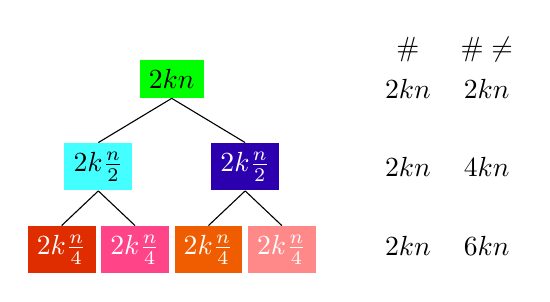
\begin{tikzpicture}
   \Tree
   [ .\node[fill=green]{$2kn$};    
       [.\node[fill=nodeblue1]{$2k\frac{n}{2}$};
           [.\node(n3l)[fill=nodered1, text=white]{$2k\frac{n}{4}$};]
           [.\node[fill=nodered2, text=white]{$2k\frac{n}{4}$};]
       ]
       [.\node[fill=nodeblue2, text=white]{$2k\frac{n}{2}$};
           [.\node[fill=nodered3, text=white]{$2k\frac{n}{4}$};]
           [.\node(n3r)[fill=nodered4, text=white]{$2k\frac{n}{4}$};]
       ]
   ]
   \node at (3,0.5) {$\#$};
   \node at (4,0.5) {$\# \neq$};
   \node at (3,0) {$2kn$};
   \node at (3,-1) {$2kn$};
   \node at (3,-2) {$2kn$};
   \node at (4,0) {$2kn$};
   \node at (4,-1) {$4kn$};
   \node at (4,-2) {$6kn$};
   \end{tikzpicture}
}
\begin{itemize}
	\item Driehoeken die in het bovenste niveau niet gesplitst kunnen worden
	\begin{itemize}
		\item Kunnen op lagere niveaus misschien wel gesplitst worden
		\item $\mathcal{O}(nlog(n))$ verschillende splitsingsvlakken ipv $\mathcal{O}(n)$
	\end{itemize}
\end{itemize}
\end{frame}

%%
%%  SECTION 4 - Implementatie
%%
\section{Implementatie}

\begin{frame}{Implementatie}
	\begin{itemize}
		\item Pbrt-v3 renderer
		\item Enkel op de CPU
		\item Bouwen is niet geparallelliseerd
		\item Geïmplementeerde $\symBSP$ bomen:
			\begin{itemize}
				\item $\symKd$
				\item $\symRBSP$ en $\symRBSPKd$
				\item $\symBSPize$ en $\symBSPizefastkd$
				\item $\symBSPrandomany$, $\symBSParbitraryany$ en $\symBSPclusterany$				
			\end{itemize}
	\end{itemize}
\end{frame}

%%
%%  SECTION 5- Resultaten
%%
\section{Resultaten}

\begin{frame}{Scenes}
	\begin{figure}
		\begin{subfigure}[t]{0.25\textwidth}
		  \centering
		  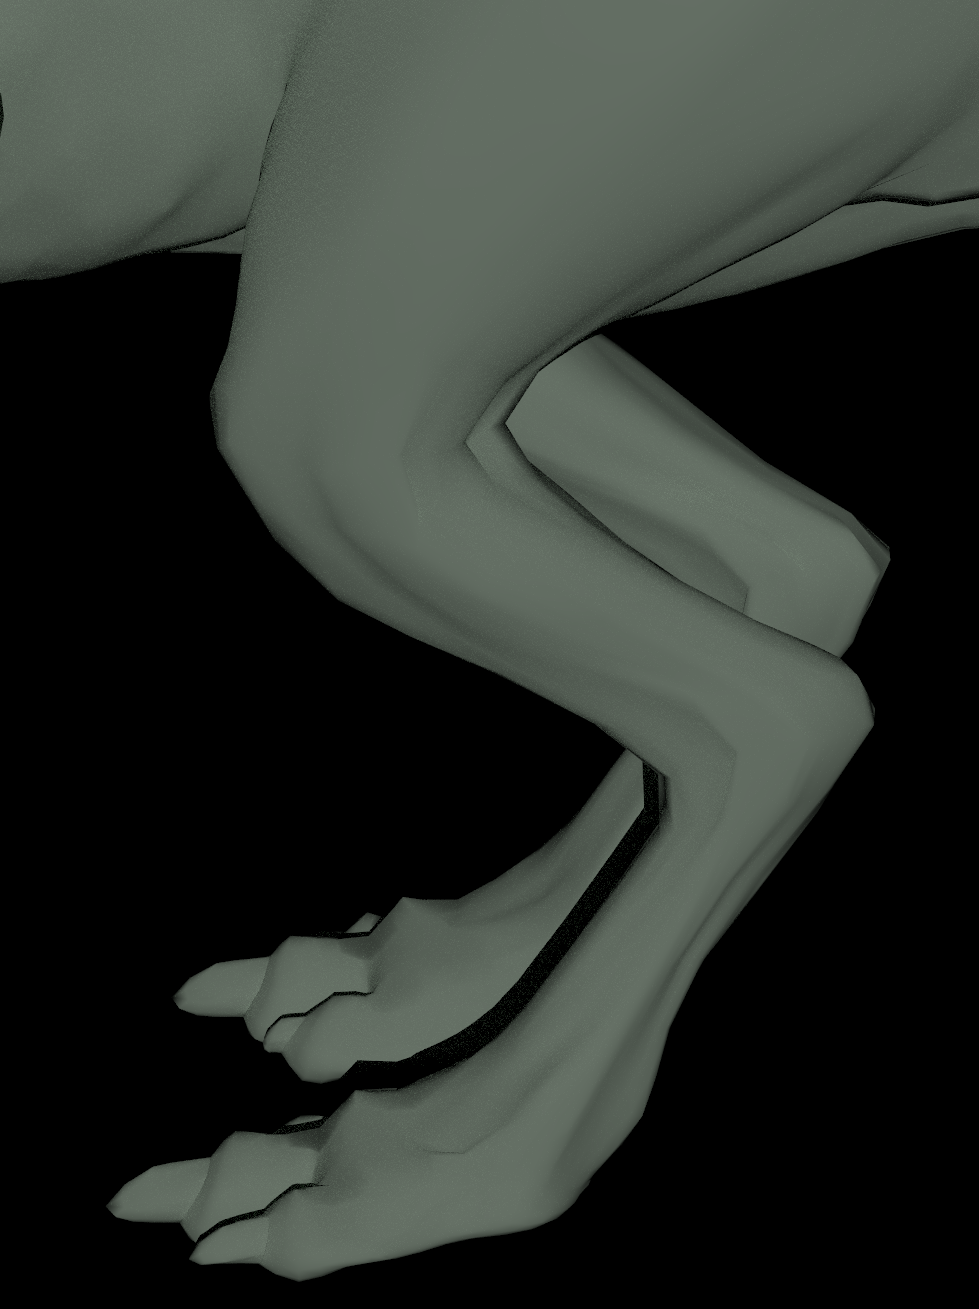
\includegraphics[width=0.6\linewidth]{../img/killerooFeet}
		  \caption{Killeroo Been scene}
		  \label{fig:results-scene-killeroo-been}    
		\end{subfigure}
		\begin{subfigure}[t]{0.20\textwidth}
		  \centering
		  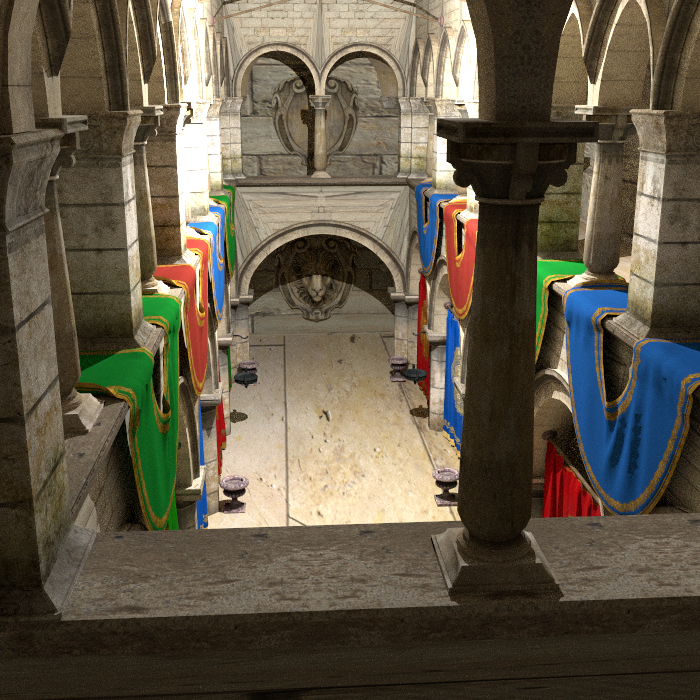
\includegraphics[width=1\linewidth]{../img/sponza}
		  \caption{Sponza scene}
		  \label{fig:results-scene-sponza}    
		\end{subfigure}
		\begin{subfigure}[t]{0.29\textwidth}
		  \centering
		  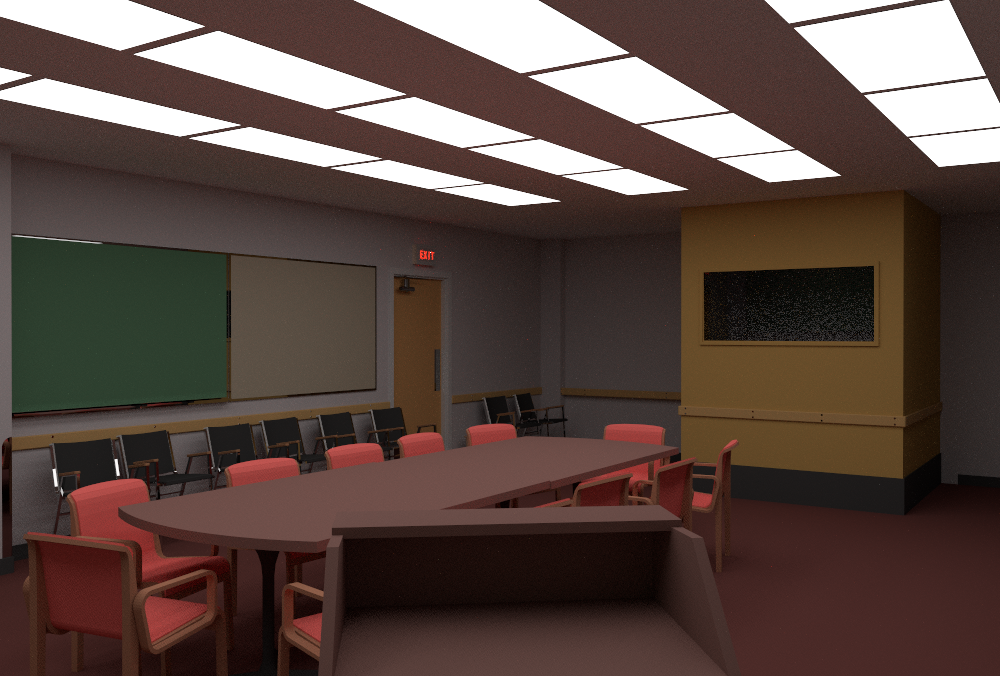
\includegraphics[width=1\linewidth]{../img/conferencehall}
		  \caption{Conference scene}
		  \label{fig:results-scene-conference}    
		\end{subfigure}
		\begin{subfigure}[t]{0.20\textwidth}
		  \centering
		  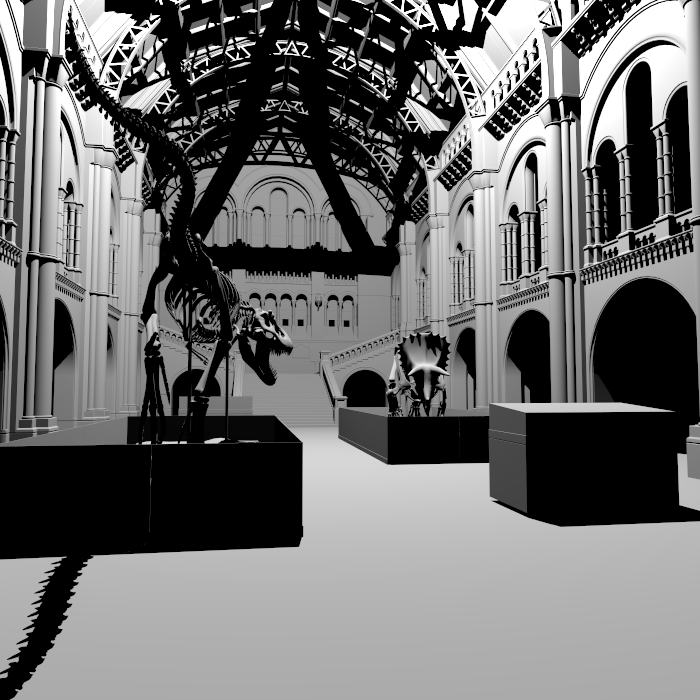
\includegraphics[width=1\linewidth]{../img/museum}
		  \caption{Museum scene}
		  \label{fig:results-scene-museum}    
		\end{subfigure}
	  \end{figure}
	  \begin{itemize}
		\item Killeroo: 33264 driehoeken
		\item Sponza: 227309 driehoeken
		\item Conference: 123651 driehoeken
		\item Museum: 1462840 driehoeken
	  \end{itemize}
\end{frame}

\begin{frame}{Twee experimenten}
	\begin{itemize}
		\item Afhankelijkheid van het aantal richtingen $k$ bij $\symBSPsweep$
		\begin{itemize}
			\item Eerste drie scenes zeven keer gerenderd
				\begin{itemize}
					\item Voor elk $k$-waarde van 2 tem 10
					\item Voor elk van de negen $\symBSPsweep$ bomen
				\end{itemize}
			\item Uitvoering met rendertijd = mediaan zeven rendertijden gebruikt als representatieve
		\end{itemize}
		\vspace{5pt}
		\item Vergelijking met de andere $\symBSP$ bomen
		\begin{itemize}
			\item Alle vier scenes zeven keer gerenderd
				\begin{itemize}
					\item Voor elke besproken bestaande $\symBSP$ boom
					\item Voor $\symBSPrandomfastkd$, $\symBSParbitraryfastkd$, $\symBSPclusterfastkd$ met optimale $k$-waarde
				\end{itemize}
			\item Uitvoering met rendertijd = mediaan zeven rendertijden gebruikt als representatieve
		\end{itemize}
	\end{itemize}
\end{frame}

\begin{frame}{Afhankelijkheid van het aantal richtingen}
	\begin{itemize}
		\item Bouwtijd
		\begin{itemize}
			\item Twee ordegroottes groter dan bouwtijd $\symKd$ boom
			\item Afhankelijkheid van $k$
				\begin{itemize}
					\item $\symBSPrandomany$ lineair
					\item $\symBSParbitraryany$ en $\symBSPclusterany$: sublineair
				\end{itemize}
			\item Op zelfde wijze afhankelijk van aantal driehoeken als $\symKd$ boom
			\item Gebruik convex veelvlak is ongeveer 25 keer trager dan asgealigneerde balk
		\end{itemize}
	\end{itemize}
\end{frame}

\begin{frame}{Afhankelijkheid van het aantal richtingen}
	\begin{itemize}
		\item Aantal knopen
		\begin{itemize}
			\item Stijgt met stijgende k, maar vlakt snel af
			\item $\symBSPrandomany$: 1.8 - 2 keer zoveel knopen als $\symKd$ boom
			\item $\symBSParbitraryany$ en $\symBSPclusterany$: 1.2 - 1.3 keer zoveel knopen als $\symKd$ boom
		\end{itemize}
		\vspace{10pt}
		\item Procentueel aantal $\symKd$ knopen
		\begin{itemize}
			\item Daalt met stijgende k, maar vlakt snel af
			\item $\symBSPrandomfastkd$: 20\% - 35 \%
			\item $\symBSParbitraryfastkd$ en $\symBSPclusterfastkd$: 30\% - 45 \%
			\item Afhankelijkheid van de diepte
				\begin{itemize}
					\item Bovenste niveaus: bijna enkel $\symKd$ knopen
					\item Onderste niveaus: bijna enkel $\symBSP$ knopen
				\end{itemize}
		\end{itemize}
	\end{itemize}
\end{frame}

\begin{frame}{Rendertijd}
		\begin{itemize}
			\item $\symBSPsweep$ boom zonder $\symKd$ richtingen
			\begin{itemize}
				\item Daalt sterk met stijgende k
				\item Enkel sneller dan $\symKd$ boom bij Killeroo Been scene
				\item Daalt tot ongeveer 1.8 keer ($\symBSPrandom$) en 1.3 keer ($\symBSParbitrary$ en $\symBSPcluster$) trager
			\end{itemize}
			\item $\symBSPsweep$ boom met $\symKd$ richtingen als $\symBSP$ richtingen
			\begin{itemize}
				\item Daalt lichtjes met stijgende k en stijgt dan voor grotere k-waarden
				\item Bij minstens één k-waarde sneller dan $\symKd$ boom
				\item $\symBSPrandomkd$ trager dan $\symBSParbitrarykd$ en $\symBSPclusterkd$
			\end{itemize}
			\item $\symBSPsweep$ boom met $\symKd$ richtingen apart behandeld
			\begin{itemize}
				\item Daalt met stijgende k
				\item Bij elk k-waarde sneller dan $\symKd$ boom
					\begin{itemize}
						\item $\symBSParbitraryfastkd$ en $\symBSPclusterfastkd$: daalt al minstens 15\% voor k = 4
					\end{itemize}
				\item $\symBSPrandomfastkd$ trager dan $\symBSParbitraryfastkd$ en $\symBSPclusterfastkd$
			\end{itemize}
		\end{itemize}
\end{frame}

\begin{frame}{Afhankelijkheid van het aantal richtingen}
	\begin{itemize}
		\item Aantal intersecties
		\begin{itemize}
			\item Verloop in functie van k zoals rendertijd
			\item $\symBSParbitraryfastkd$ en $\symBSPclusterfastkd$:
				\begin{itemize}
					\item daling tot 40\%
					\item vlak vanaf een k-waarde van 5
				\end{itemize}
			\item $\symBSPrandomfastkd$:
				\begin{itemize}
					\item daling tot 40\%
					\item daalt trager maar monotoon in functie van k
				\end{itemize}
		\end{itemize}
	\end{itemize}
\end{frame}

\begin{frame}{Afhankelijkheid van het aantal richtingen}
	\begin{itemize}
		\item Aantal doorkruisingen
		\begin{itemize}
			\item $\symBSParbitraryfastkd$ en $\symBSPclusterfastkd$:
				\begin{itemize}
					\item evenveel als $\symKd$ boom
					\item onafhankelijk van k
				\end{itemize}
			\item $\symBSPrandomfastkd$:
				\begin{itemize}
					\item stijgt tot 10\% meer dan $\symKd$ boom
					\item stijgt traag en monotoon in functie van k
				\end{itemize}
		\end{itemize}
		\item Procentueel aantal $\symKd$ doorkruisingen
		\begin{itemize}
			\item $\symBSParbitraryfastkd$ en $\symBSPclusterfastkd$:
				\begin{itemize}
					\item 85\% - 90\%
					\item vlak vanaf k-waarde van 5
				\end{itemize}
			\item $\symBSPrandomfastkd$:
				\begin{itemize}
					\item 80\% - 90\%
					\item daalt traag en monotoon in functie van k
				\end{itemize}
		\end{itemize}
	\end{itemize}
\end{frame}

\begin{frame}{Vergelijking bestaande bomen}
	\begin{itemize}
		\item Nieuwe bomen
		\begin{itemize}
			\item $\symBSPrandomfastkd$ met k = 10
			\item $\symBSParbitraryfastkd$ met k = 6
			\item $\symBSPclusterfastkd$ met k = 6
			\item $\symRBSPKd$ met k = 13
		\end{itemize}
		\item Bestaande bomen
		\begin{itemize}
			\item $\symKd$
			\item $\symRBSP$ met k = 13
			\item $\symBSPize$
			\item $\symBSPizefastkd$
		\end{itemize}
	\end{itemize}
\end{frame}

\begin{frame}[c]{Rendertijd en Bouwtijd}
	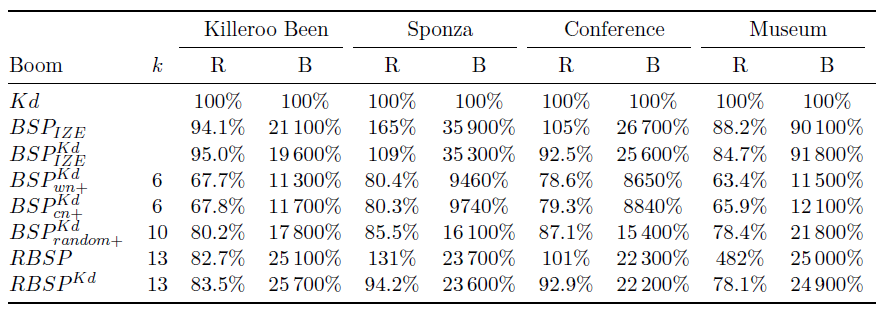
\includegraphics[width=.9\paperwidth]{graphics/rendertijd}
\end{frame}

\begin{frame}[c]{Straal-driehoekintersecties}
	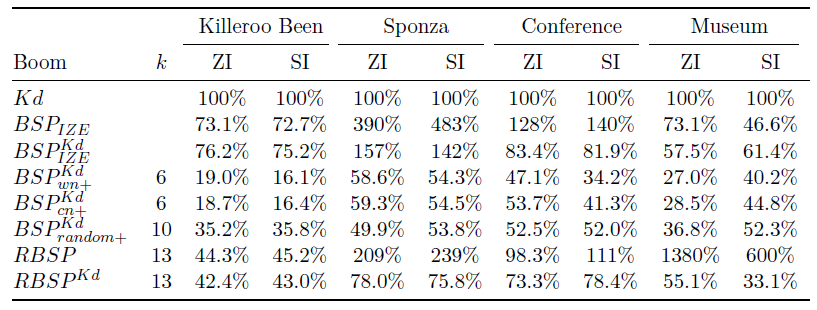
\includegraphics[width=.9\paperwidth]{graphics/intersecties}
\end{frame}

\begin{frame}[c]{\textit{False color} afbeeldingen intersecties}
	\begin{itemize}
		\item $\symBSParbitraryfastkd$ vs $\symKd$
	\end{itemize}
	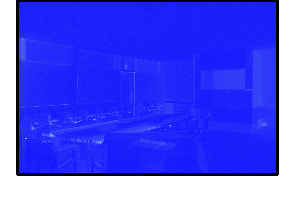
\includegraphics[height=.35\paperheight]{../img/fc/conference/bsparbitraryfastkd}
	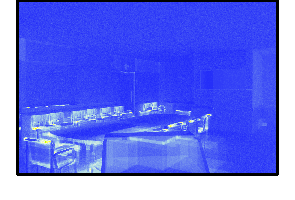
\includegraphics[height=.35\paperheight]{../img/fc/conference/kdtree}
	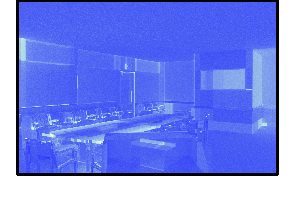
\includegraphics[height=.35\paperheight]{../img/fc/conference/own-bsparbitraryfastkd}
	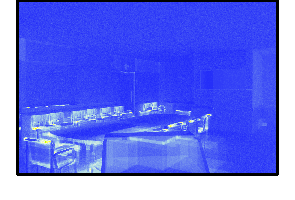
\includegraphics[height=.35\paperheight]{../img/fc/conference/own-kdtree}
\end{frame}

\begin{frame}[c]{Inwendige knoopdoorkruisingen}
	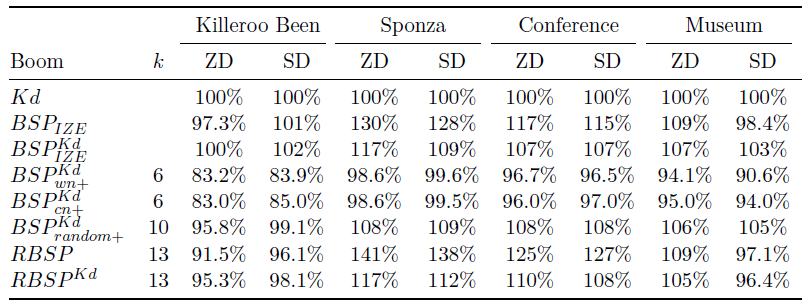
\includegraphics[width=.9\paperwidth]{graphics/doorkruisingen}
\end{frame}

\begin{frame}[c]{$\symKd$ knoopdoorkruisingen}
	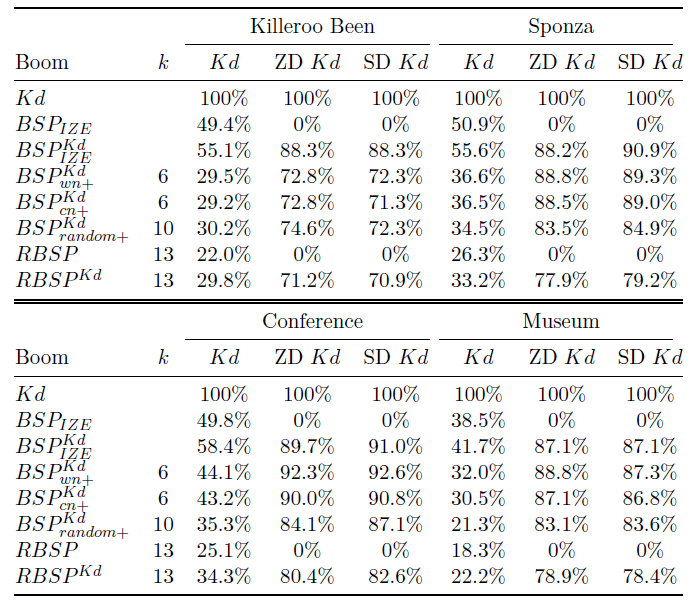
\includegraphics[height=.75\paperheight]{graphics/kdknopen}
\end{frame}

%%
%%  SECTION 6- Conclusie
%%
\section{Conclusie}

\begin{frame}{Conclusie}
	\begin{itemize}
		\item $\symBSPsweep$
		\begin{itemize}
			\item Nuttig en uitbreidbaar concept voor algemene $\symBSP$ bomen
			\item Lokale geometerie makkelijk in rekening te brengen
			\item Beperkte bouwtijd door \textit{sweeping}
		\end{itemize}
		\item Variant met snelle $\symKd$ richtingen is superieur
		\item $\symBSPrandomfastkd$
			\begin{itemize}
				\item In elke knoop andere splitsingsvlakken kiezen maakt de boom beter
			\end{itemize}
		\item $\symBSParbitraryfastkd$ en $\symBSPclusterfastkd$
			\begin{itemize}
			\item Splitsingsvlakken afhankelijk van lokale geometrie (normalen) maken de boom nog beter
			\item Vermindering rendertijd met meer dan 20\%
			\item Vermindering straal-driehoekintersecties met meer dan 40\%
			\item Clustering lijkt geen voordeel te bieden
			\end{itemize}

	\end{itemize}
\end{frame}

\begin{frame}{Toekomstig onderzoek}
	\begin{itemize}
		\item Verbeteren bouwtijd
		\item Bepalen beste aantal richtingen (per diepte)
		\item Bepalen betere richtingen
		\item Focus op splitsen in disjuncte delen ipv SA kost
	\end{itemize}
\end{frame}


\begin{frame}[c,plain,noframenumbering]
	\begin{tikzpicture}[remember picture,overlay]
	\fill[fill=kul-blue]
		(current page.south east)  rectangle  ([shift={(0,-0.1\paperheight)}]current page.north west)   ;
	\end{tikzpicture}
	
	\centering
	\textcolor{white}{Bedankt voor jullie aandacht}
	\end{frame}

\end{document}